% =====================================================================
%  Chapter 6 -- Stage 3: the experiment in software (staircase in R_F)
% =====================================================================
\chapter{Stage 3: The Experiment in Software}\label{ch:stage3}
\chapterlists

The fastest useful bench sweep in configuration A was about \SI{9}{\kilo\ohm\per\second}. To see what
happens far beyond it, we reproduced Stage~2 step for step in simulation and pushed the rate more than
ten times higher.

\section{What we did}\label{sec:s3-setup}

The simulated circuit (\cref{sec:simulation}) follows the Arduino staircase exactly: 32 levels from
\num{91} to \SI{101}{\kilo\ohm}, each held for $\tau$, after the same trigger pulse. Forty-three rates
from \SI{52}{\ohmpersec} to \SI{103}{\kilo\ohm\per\second} were simulated and analysed like the bench data.
Here $\Gc=3$ ($\RF=\SI{94}{\kilo\ohm}$) and $\Asat=\SI{13.9}{\volt}$.

\section{What we saw}\label{sec:s3-results}

\subsection{At bench rates}

The simulation reproduces the bench (\cref{fig:s3-recordings}, top; \cref{fig:s3-thresholds}a). For the
23 rates below \SI{4.2}{\kilo\ohm\per\second},
\begin{align}
  \Ron  &= (\num{93934 \pm 18})\,\si{\ohm} + (\num{52.4 \pm 0.4})\sqrt{\lambda} , \label{eq:s3-on}\\
  \Roff &= (\num{94006 \pm 4})\,\si{\ohm} - (\num{30.30 \pm 0.08})\sqrt{\lambda} . \label{eq:s3-off}
\end{align}
The switch-off intercept is within \SI{6}{\ohm} of the ideal threshold and $k_{\mathrm{off}}$ within about
$1\%$ of \cref{eq:koff-value}; free exponents are $0.485\pm0.007$ (off) and $0.51\pm0.02$ (on).

\begin{figure}[!htb]
  \centering
  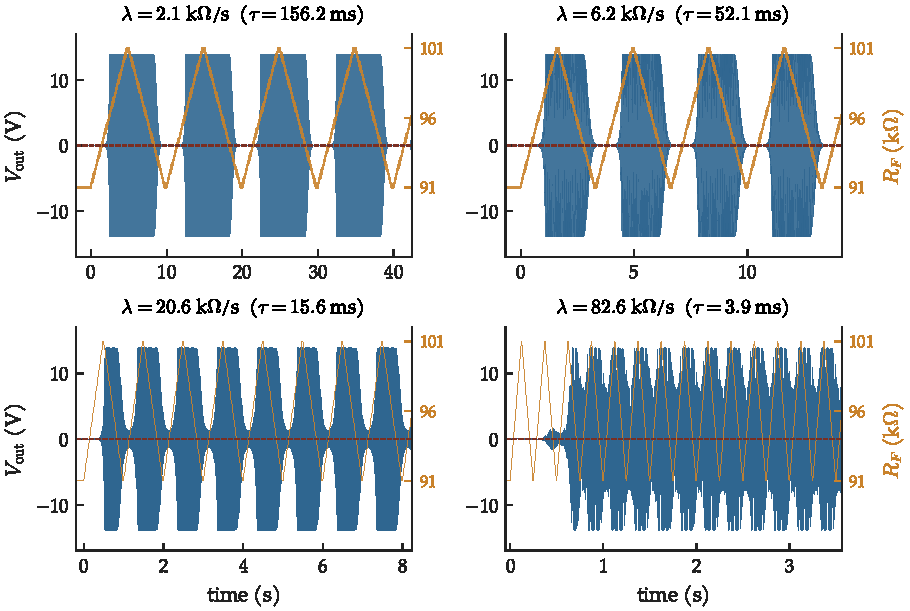
\includegraphics[width=\linewidth]{fig_s3_recordings}
  \caption[Stage 3: simulated recordings]{Stage 3: simulated recordings. At \num{2.1} and
  \SI{6.2}{\kilo\ohm\per\second} bursts are separate, as on the bench; at \SI{20.6}{\kilo\ohm\per\second}
  the oscillation no longer dies fully between bursts; at \SI{82.6}{\kilo\ohm\per\second} it never
  switches off.}
  \label{fig:s3-recordings}
\end{figure}

\begin{figure}[!htb]
  \centering
  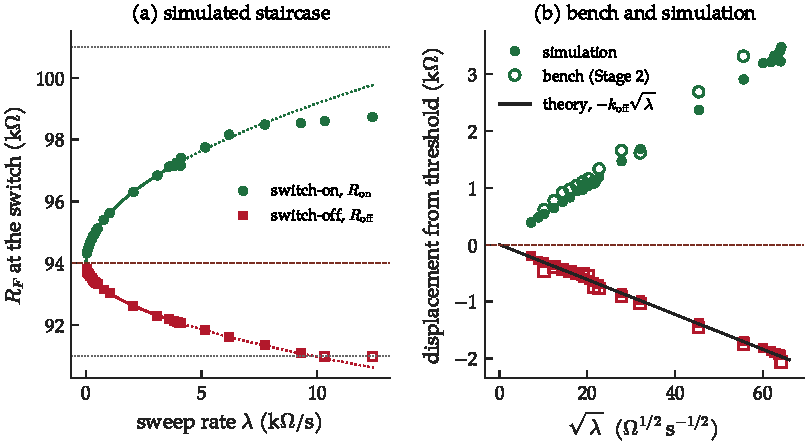
\includegraphics[width=\linewidth]{fig_s3_thresholds}
  \caption[Stage 3: switching points in simulation]{Stage 3: (a)~simulated switching points with
  \cref{eq:s3-on,eq:s3-off} (dotted: extrapolation; open squares: decay completed only after the sweep
  turned). (b)~Displacement from threshold against $\sqrt{\lambda}$, simulation (filled) and bench (open);
  black: parameter-free switch-off prediction.}
  \label{fig:s3-thresholds}
\end{figure}

Measured from their own thresholds, bench and simulation fall on the same lines
(\cref{fig:s3-thresholds}b, \cref{tab:s3-compare}). The only real difference is the threshold itself,
\SI{97.4}{\kilo\ohm} against \SI{94.0}{\kilo\ohm}, i.e.\ the shift of $\Gc$ from 3 to 3.07
(\cref{eq:s2-Gc}). The smaller simulated $k_{\mathrm{on}}$ reflects a larger effective noise floor
($\Lon=6.7$).

\begin{table}[!htb]
  \centering
  \small
  \setlength{\tabcolsep}{4pt}
  \begin{tabular}{@{}lccc@{}}
    \toprule
    & \textbf{Bench} (Stage 2) & \textbf{Simulation} (Stage 3) & \textbf{Theory} \\
    \midrule
    Threshold $R_{c}$ (switch-off fit) & \SI{97.47}{\kilo\ohm} & \SI{94.01}{\kilo\ohm} & \SI{94.00}{\kilo\ohm} (ideal) \\
    Threshold gain $\Gc$ & 3.07 & 3.00 & 3 \\
    $k_{\mathrm{off}}$ (\si{\ohm^{1/2}\,\second^{1/2}}) & \num{31.8 \pm 1.1} & \num{30.30 \pm 0.08} & 30.6, \cref{eq:koff-value} \\
    $k_{\mathrm{on}}$ (\si{\ohm^{1/2}\,\second^{1/2}}) & \num{58.1 \pm 2.2} & \num{52.4 \pm 0.4} & 54 to 69, \cref{tab:kon} \\
    $k_{\mathrm{on}}/k_{\mathrm{off}}$ & 1.83 & 1.73 & $\sqrt{\Lon/\Loff}$, \cref{eq:k-ratio} \\
    \bottomrule
  \end{tabular}
  \caption[Bench and simulation compared]{The $\sqrt{\lambda}$ laws on the bench, in simulation, and in
  theory.}
  \label{tab:s3-compare}
\end{table}

\subsection{Beyond bench rates: a second critical rate}

At \SI{20.6}{\kilo\ohm\per\second} (\cref{fig:s3-recordings}) the oscillation no longer falls back to
noise between bursts; at \SI{82.6}{\kilo\ohm\per\second} it stays on, although the gain still dips below
threshold every cycle. This is regime (b) of \cref{sec:budget}: here $\Gp>\Gm$
(\cref{tab:budget-theory}), so the decay budget runs out first. \Cref{eq:Amin,eq:budget-rate} predict,
with no free parameter, $A_{\min}/\Asat=e^{-\Gm}$; above \SI{15}{\kilo\ohm\per\second} the simulation agrees
with this to within about $2\%$ (\cref{fig:s3-amin}).

\begin{figure}[!htb]
  \centering
  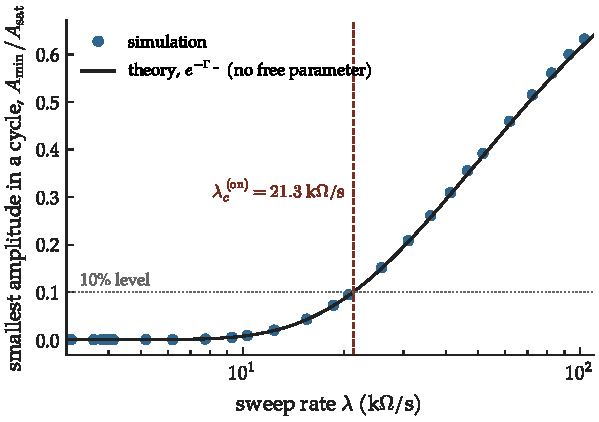
\includegraphics[width=0.62\linewidth]{fig_s3_amin}
  \caption[Stage 3: the oscillation stops switching off]{Stage 3: smallest amplitude per cycle against
  rate. Points: simulation. Line: parameter-free $e^{-\Gm}$ (\cref{eq:Amin,eq:budget-rate}). Above the
  second critical rate (dashed) the minimum stays above 10\% and the circuit no longer switches off.}
  \label{fig:s3-amin}
\end{figure}

The minimum crosses the 10\% switch-off level between the runs at \num{20.6} and
\SI{25.8}{\kilo\ohm\per\second}, at about \SI{21.1}{\kilo\ohm\per\second} by interpolation, against the
prediction of \cref{eq:lamc-on},
\begin{equation}
  \lambda_{c}^{\text{(on)}} = \SI{21.3}{\kilo\ohm\per\second} .
  \label{eq:s3-lamc}
\end{equation} Above this rate the long-time state changes from bursting to permanent
oscillation. The loops show the same (\cref{fig:s3-loops}): narrow at slow rates, four times wider at
\SI{2}{\kilo\ohm\per\second}, and at \SI{46}{\kilo\ohm\per\second} never closing, the lower branch
bottoming out at about a third of full size.

\begin{figure}[!htb]
  \centering
  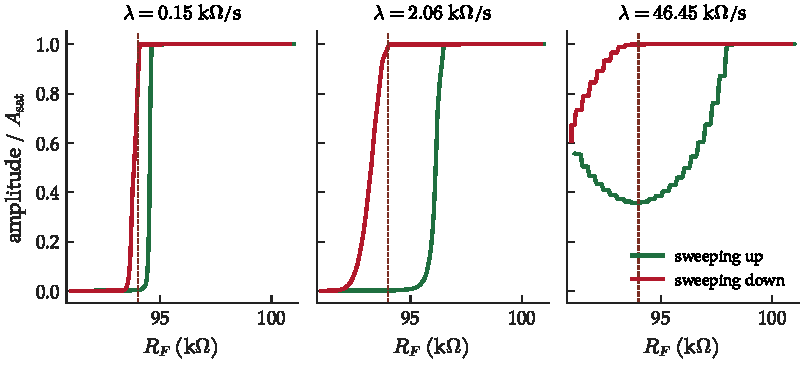
\includegraphics[width=\linewidth]{fig_s3_loops}
  \caption[Stage 3: simulated hysteresis loops]{Stage 3: simulated loops. At \SI{46}{\kilo\ohm\per\second}
  the amplitude never falls below about 35\%: permanently on.}
  \label{fig:s3-loops}
\end{figure}

\section{What this stage taught us}\label{sec:s3-learned}

\begin{learned}
\begin{itemize}[leftmargin=1.2em]
  \item \textbf{The simulation reproduces the bench}; the only significant difference is the real
        threshold.
  \item \textbf{The long-time state can depend on the rate}: bursting below about
        \SI{21}{\kilo\ohm\per\second}, always on above, in parameter-free agreement with the budget theory.
  \item \textbf{This is out of bench reach} in configuration A: at \SI{21}{\kilo\ohm\per\second} each step
        lasts \SI{15}{\milli\second}, about one period.
\end{itemize}
\end{learned}

The growth budget suggested a way out. Sweeping $\Ri$ doubles the gain change per step
(\cref{tab:configs}) and reverses the balance of the budgets, so the fast-rate state becomes ``off for
good'' (\cref{tab:budget-theory}); with the measured bench threshold, the predicted critical rate also
falls within bench reach. This is configuration B.
